\documentclass{report}
\title{Thesis proposal: Understanding Outdoor Photometric Stereo}
\author{Yannick Hold-Geoffroy}
%\programme{Doctorat en g\'enie \'electrique}
%\annee{2015}


\date{\today}

%\usepackage{hyperref}
%\hypersetup{colorlinks,allcolors=ULlinkcolor}

%\frenchbsetup{%
%  CompactItemize=false,         % ne pas compacter les listes
%  ThinSpaceInFrenchNumbers=true % espace fine dans les nombres
%}


\usepackage[letterpaper, margin=1in]{geometry}
\usepackage[utf8]{inputenc}
\usepackage{times}
\usepackage{amsmath}
\usepackage{amssymb}
%\bibliographystyle{unsrtnat}
\usepackage[numbers,sort&compress]{natbib}
%\usepackage[numbers]{natbib}
%\usepackage{cite}   % sort citation numbers automatically
\usepackage{notoccite}
\usepackage{url}
\usepackage{graphicx}
\usepackage{rotating}
\usepackage{gensymb}
\usepackage{xcolor}
\usepackage{nicefrac}
%\usepackage{adjustbox}
%\usepackage{authblk}
% to control spacing in item lists
\usepackage[titletoc]{appendix}
\usepackage{enumitem}
\usepackage[pagebackref=false,breaklinks=true,colorlinks=true,linkcolor=black,bookmarks=true]{hyperref}
\usepackage{defs}
\usepackage{amsmath,esint}

\linespread{1.5}


\begin{document}

%\frontmatter                    % pages liminaires

\maketitle
%\pagetitreonlyone                     % production des pages de titre

\tableofcontents

\hypersetup{colorlinks=true,linkcolor=blue}

% Commands
\newcommand*\B[1]{\mathbf{#1}}
\newcommand{\boldomega}{\boldsymbol \omega} % bold omega
\newcommand{\boldmu}{\boldsymbol \mu} % bold omega
\newcommand{\bolddelta}{\boldsymbol \delta} % bold delta

\newcommand\norm[1]{\left\lVert#1\right\rVert}

\newcommand\todo[1]{\textcolor{red}{TODO: #1}}

\graphicspath{{figures/}}

\chapter{Questions by Denis Laudenreau}

\section*{Question 1}

\subsection{(a)}

Suppose q as the distance between the strip light and P along the x-axis.

\begin{equation}
E(r) = \frac{1}{\pi} \int_{\Omega} L(r,\omega)\cos(\theta) d\omega
\end{equation}
\begin{align*}
E(r) &= \frac{1}{\pi} \int_{-\arctan(\frac{\frac{H}{2}}{\sqrt{q^2+r^2}})}^{\arctan(\frac{\frac{H}{2}}{\sqrt{q^2+r^2}})} \int_{0}^{\arctan(\frac{w}{q})} L(r,\omega)\cos(\theta) \sin(\theta) d\theta d\phi \\
     &= 2 \cdot \arctan(\frac{\frac{H}{2}}{\sqrt{q^2+r^2}}) \cdot \int_{\arctan(\frac{q}{r-W/2})}^{\arctan(\frac{q}{r+W/2})} L(r,\omega)\cos(\theta) \sin(\theta) d\theta \\
     &= 2 \cdot \arctan(\frac{H}{2\sqrt{q^2+r^2}}) \cdot \left[ - \frac{1}{2} \cos^2(x) \right]_{\arctan(\frac{q}{r-W/2})}^{\arctan(\frac{q}{r+W/2})} \\
     &= 2 \cdot \arctan(\frac{H}{2\sqrt{q^2+r^2}}) \cdot \left[ - \frac{1}{2} \cos^2(\arctan(\frac{q}{r+W/2})) - - \frac{1}{2} \cos^2(\arctan(\frac{q}{r-W/2})) \right] \\
\end{align*}

\subsection{(b)}

As H gets bigger, the integral along the elevation axis gets closer toward $\pi$.

\subsection{(c)}



\section{Question 2}
\subsection{(a)}

$\Omega$
\begin{equation}
E(r) = \frac{1}{\pi} \int_{\Omega} L(r,\omega)\cos(\theta) d\omega
\end{equation}
\begin{align*}
E(r) &= \frac{1}{\pi} \int_{0}^{\arctan(\frac{h}{q})} \int_{0}^{\arctan(\frac{w}{q})} L(r,\omega)\cos(\theta) \sin(\theta) d\theta d\phi \\
     &= \arctan(\frac{h}{q}) \cdot \int_{0}^{\arctan(\frac{w}{q})} L(r,\omega)\cos(\theta) \sin(\theta) d\theta \\
     &= \arctan(\frac{h}{q}) \cdot \left[ - \frac{1}{2} \cos^2(x) \right]_{0}^{\arctan(\frac{w}{q})} \\
     &= \arctan(\frac{h}{q}) \cdot \left[ - \frac{1}{2} \cdot \cos^2(\arctan(\frac{w}{q})) - -\frac{1}{2} \right] \\
\end{align*}


\begin{equation}
E(r) = \frac{M}{2\pi} \sum_{i=1}^{n} \beta_i \cos(\alpha_i)
\end{equation}
\begin{align*}
E(r) = \frac{M}{2\pi} \left( \arctan(\frac{w}{q}) + \arctan(\frac{h}{q}) + \arctan(\frac{w}{q}) \cdot \cos(\arctan(\frac{h}{q})) + \arctan(\frac{w}{q}) \cdot \cos(\arctan(\frac{w}{q})) \right)
\end{align*}

\subsection{(b)}

\chapter{Questions by Philippe Giguère}

\section{Question 3}

Setup: Graphique

For this setup, each light generate a row $\B{l}$ in the lighting matrix $\B{L}$ as such:
\begin{equation}
\B{l} =
\left[\begin{array}{c} \cos\!\left(\theta\right)\, \sin\!\left(r\right) \\ \sin\!\left(r\right)\, \sin\!\left(\theta\right) \\ \sqrt{ - {\cos\!\left(\theta\right)}^2\, {\sin\!\left(r\right)}^2 - {\sin\!\left(r\right)}^2\, {\sin\!\left(\theta\right)}^2 + 1} \end{array}\right]^T
\quad .
\end{equation}

In the current setup, the lights are $120\degree$ apart on the $xy$-plane, so $\theta = \left[ 0\degree, 120\degree, 240\degree \right]$. This translates in the following lighting matrix:
\begin{equation}
\B{L} =
\left[\begin{array}{ccc} \sin\!\left(r\right) & 0 & \sqrt{1 - {\sin\!\left(r\right)}^2}\\ -\frac{\sin\!\left(r\right)}{2} & \frac{\sqrt{3}\, \sin\!\left(r\right)}{2} & \sqrt{1 - {\sin\!\left(r\right)}^2}\\ -\frac{\sin\!\left(r\right)}{2} & -\frac{\sqrt{3}\, \sin\!\left(r\right)}{2} & \sqrt{1 - {\sin\!\left(r\right)}^2} \end{array}\right]
\quad .
\end{equation}

Given the simple lambertian reflectance equation, we can compute the pixel intensity of a camera pointed directly to a surface with normal $\B{n}$:
\begin{equation}
b = \B{L}\B{n}
\quad.
\end{equation}

Photometric Stereo finds the normals $\B{n} = \left[ n_x \; n_y \; n_z\right]^T$ back from the lighting matrix $\B{L}$ and the pixel intensity $b$. This can be done by inverting the light matrix $\B{L}$, hence performing a least squares fit to the problem, as such:
\begin{equation}
\B{L}^{-1}\B{b} = \B{n} = 
\begin{bmatrix}
n_x \\
n_y \\
n_z 
\end{bmatrix}
\quad.
\end{equation}
We can see that, unless matrix $\B{L}$ is singular and exempt of noise, we retrieve the three components of the normal $\B{n}$ directly.

But, instead of solving the usual equation, we have a systematic error $\epsilon_r$ in the measurement of $r$, making the noisy lighting matrix $\B{L}_\epsilon$ a bit different that the original matrix:
\begin{equation}
\B{L}_\epsilon = \left[\begin{array}{ccc} \sin\!\left(\epsilon_r + r\right) & 0 & \sqrt{1 - {\sin\!\left(\epsilon_r + r\right)}^2}\\ -\frac{\sin\!\left(\epsilon_r + r\right)}{2} & \frac{\sqrt{3}\, \sin\!\left(\epsilon_r + r\right)}{2} & \sqrt{1 - {\sin\!\left(\epsilon_r + r\right)}^2}\\ -\frac{\sin\!\left(\epsilon_r + r\right)}{2} & -\frac{\sqrt{3}\, \sin\!\left(\epsilon_r + r\right)}{2} & \sqrt{1 - {\sin\!\left(\epsilon_r + r\right)}^2} \end{array}\right]
\quad.
\end{equation}
Solving this problem gives us:
\begin{equation}
\B{L}_\epsilon^{-1}\B{b} = \B{n}_\epsilon = 
\left[\begin{array}{c} n_x \cdot \frac{\sin\!\left(r\right)}{\sin\!\left(\epsilon_r + r\right)}\\ n_y \cdot \frac{\sin\!\left(r\right)}{\sin\!\left(\epsilon_r + r\right)}\\ n_z \cdot \frac{\sqrt{1 - {\sin\!\left(r\right)}^2}}{\sqrt{1 - {\sin\!\left(\epsilon_r + r\right)}^2}} \end{array}\right]
\quad,
\end{equation}
where the normal components $n_x$, $n_y$ and $n_z$ are all multiplied by a non-unit factor due to the measurement error $\epsilon_r$.

``Inversion error, condition number and approximate inverses of uncertain matrices, eq 1.1''

\section{Question 4}

\chapter{Questions by Paulo Gotardo}

\section{Question 5}
\subsection{(a)}
\textbf{Let $\B{A} \in \mathbb{R}^{m \times n}$, with $m \gg n$. Show how the eigenvalues and (unit) eigenvectors of $\B{AA}^T$ can be obtained from the eigen decomposition of the smaller matrix $\B{A}^T\B{A}$.}

By the definition of the Singular Value Decomposition (SVD), any matrix real $A$ can be factored such as
\begin{equation}
\B{A} = \B{U \Sigma V}^T \quad.
\end{equation}
Matrices $\B{U}$, $\B{\Sigma}$ and $\B{V}$ are closely related to the eigen decomposition. First, $\Sigma$ is a diagonal matrix yielding the singular values of $A$, which are the square roots of the eigenvalues of both $\B{AA}^T$ and $\B{A}^T\B{A}$. Second, the columns of $\B{U}$ and $\B{V}$ are, by definition, the eigenvectors of $\B{AA}^T$ and $\B{A}^T\B{A}$, respectively. We can convince ourselves of both with these relations:
\begin{align*}
\B{AA}^T           &= \B{V\Sigma}^T\B{U}^T \; \B{U\Sigma V}^T
                        &&= \B{V\Sigma}^T\B{IU\Sigma V}^T 
                        &&&= \B{V\Sigma}^T\B{\Sigma V}^T \quad,\\
\B{A}^T\B{A}  &= \B{U\Sigma V}^T \; \B{V\Sigma}^T\B{U}^T
                        &&= \B{U\Sigma V}^T \; \B{V\Sigma}^T\B{U}^T
                        &&&= \B{U\Sigma}\B{\Sigma}^T\B{U}^T \quad.
\end{align*}
As the columns of $\B{U}$ and $\B{V}$ are a orthonormal basis (as they hold the eigenvectors), both $\B{U}^T\B{U}^T$ and $\B{V}^T\B{V}$ gives the identity matrix $\B{I}$ as result.

Two relationships are sought in the question: the eigenvalues and eigenvectors of both pre and post multiplication by the transpose. First, the relationship between the eigenvalues of $\B{A}^T\B{A}$ and $\B{AA}^T$ is pretty simple: they are the same. On the other hand, both their eigenvectors is only related through $\B{A}$:
\begin{align*}
\B{A}  &= \B{U \Sigma V}^T \\
\B{AV} &= \B{U \Sigma V}^T \B{V} = \B{U \Sigma I} \\
\B{AV\Sigma}^\dagger &= \B{U \Sigma \Sigma}^\dagger = \B{U} \quad,
\end{align*}
where $\B{\Sigma}^\dagger$ is the pseudoinverse of $\B{\Sigma}$. This $\B{\Sigma}^\dagger$ is used as a normalization factor for the $\B{AV}$ matrix; normalizing each column of $\B{AV}$ would produce the same result.

This relation will provide as many eigenvectors as there are linearly independent vectors of $\B{AA}^T$. Since $m \gg n$, this means that at most $n$ eigenvectors of $\B{AA}^T$ will be found. The rest of the resulting matrix will contain only zeros. The vectors that are missing compose the null space of $\B{A}^T$ (and $\B{AA}^T$).

\subsection{(b)}
\subsection{(c)}
\section{Question 6}
``Take a look at this paper (if you haven't done that already). The intro makes a very good point: color variation in natural illumination is a form of (single-image) photometric stereo.

Translation: we could compute 3 MLVs per image (one per color channel). Wonder how much cloud coverage changes the color of sun light.
Paper SENI''
\section{Question 7}

Granados 2010 / 2013

\chapter{Questions by Jean-François Lalonde}

\section{Question 8}
\subsection{(a)}
\textbf{Given a known lighting environment map $\B{L}$ (e.g.\ in latitude-longitude representation), explain how SH coefficients $s$ can be estimated from $\B{L}$.}

Each SH coefficients $s$ is linked to a basis function of order $n$ and mode $m$ defined over the sphere. These coefficients are computed by projecting the environment map $\B{L}$ on the according function, called $Y_n^m$:
\begin{equation}
\oiint\limits_{\Omega} \B{L}\left(\B{\omega} \right) Y_n^m \left( \B{\omega} \right) \mathrm{d} \B{\omega}   \quad.
\end{equation}

In the discrete case, just like the environment map $\B{L}$, these functions can be represented in latitude-longitude representation. This allows the projection to be performed as the summation of its pixelwise multiplication with the environment map $\B{L}$:
\begin{equation}
\sum_{v=0}^{h} \sum_{u=0}^{w} \B{L}_{u,v} Y_n^m\left(u, v\right) \omega_{u,v}^2 \quad,
\end{equation}
for an environment map $\B{L}$ of width $w$ and height $h$. The solid angle subtended by pixel $u,v$, called $\omega_{u,v}$ is required to weight accordingly each pixel of both maps. Because of the latitude-longitude representation, each pixel covers a different surface area over the sphere. Without this solid angle weighting, pixels near the top and bottom edge of the environment map are more important, resulting in a brighter  [...].

\begin{figure}[hb]
  \centering
  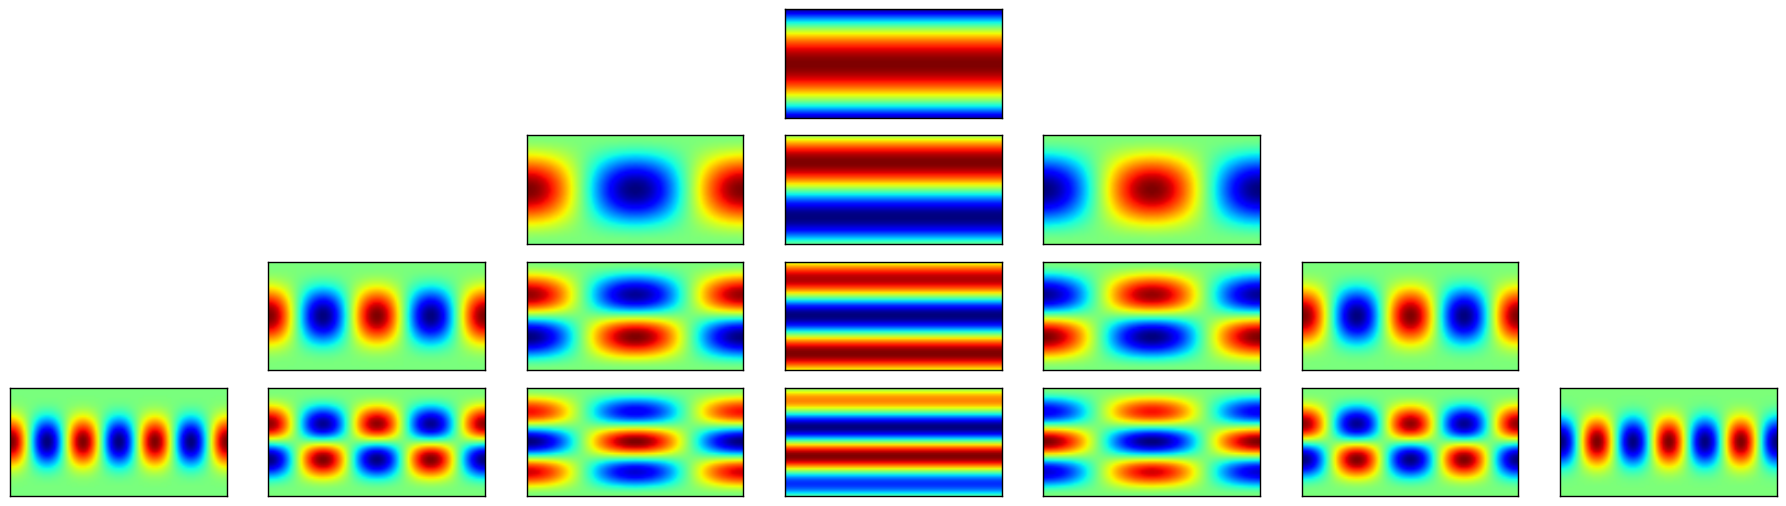
\includegraphics[width=0.45\linewidth]{q8_a_pyramid_real.png}
  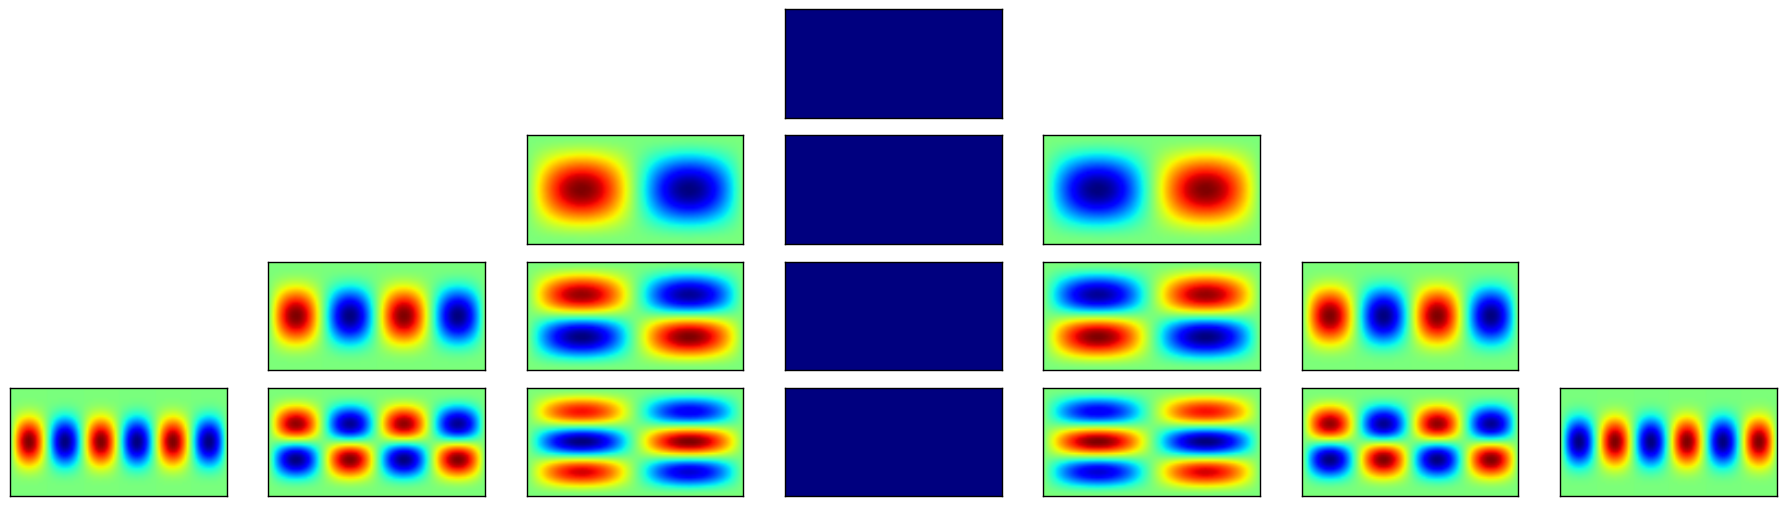
\includegraphics[width=0.45\linewidth]{q8_a_pyramid_imag.png}
  \caption[Sample Spherical Harmonics]
   {Basis of degrees 0-3 of Spherical Harmonics}
\end{figure}

%Just like the Fourier transform, Spherical Harmonics is a transform using a principal root of unity as its kernel. Having a kernel based on a principal root of unity over the function's domain confers a plethora of interesting attributes. One of which is that the functions generated form an orthonormal basis spanning the whole domain, called a complete orthonormal system.

This pixelwise multiplication works because the SH basis forms an orthonormal system. Projecting something on an orthonormal basis can be called a dot product, because it yields the same properties. Thus, this relation holds \emph{iif} $f(x)$ and $g(x)$ are orthogonal over period $p$:
\begin{equation}
f \cdot g=\int_{-p}^p f(x)g(x)\,dx\ \quad,
\end{equation}
explaining why discrete transforms in general (SH, Fourier, Z, etc.) work using a single per-element multiplication.

%Computing a coefficient $s$ of a given order $n$ and mode $m$ of spherical harmonic is be done by projecting the base $Y_n^m$ on the environment map $\B{L}$. Given a latitude-longitude representation,

\subsection{(b)}
Approximation, cos, Stupid SH tricks
\subsection{(c)}
HH paper
\subsection{(d)}
Stupid SH tricks
\section{Question 9}

{\small
\bibliographystyle{acm}
\bibliography{library}
}

\end{document}
